%%%%%%
%This files creates a pdf file of "The Deterministic Spider:
%A Benchmark for Evaluating Efficiency of
%Swarms Search". This abstract will
%be submitted to the 2015 IROS Conference. Final Abstract
%due on Aug 31, 2015.
%%%%%%

%%%%%
%Preamble
%This specifies the page layout and packages.
%%%%%
\documentclass[10pt]{article}
\usepackage[margin=0.75in, paperwidth=8.5in, paperheight=11in]{geometry}
\usepackage{graphicx}
\usepackage{wrapfig}
\usepackage{natbib}
\usepackage{caption}
\usepackage{subcaption}
\usepackage[utf8]{inputenc}
       \usepackage[T1]{fontenc}
       \usepackage{lmodern}
       \usepackage{graphicx}
       \usepackage{caption}
        \usepackage{floatrow}%
\usepackage{titling}
%%%%%
%Article title and authors, and header stuff
%%%%%
% \setlength{\droptitle}{-14em}  
% \title{\vspace{-0.5cm}\large\textbf{The Deterministic Spider: A Benchmark for Evaluating Efficiency of Swarm Search}}\vspace{-5pt}
% \author{\small Linh T. Tran, G. Matthew Fricke, Joshua P. Hecker, and Melanie E. Moses}\setlength{\droptitle}{-18pt}
% \date{}
\begin{document}

%Title
\begingroup  
  \centering
  \large \textbf{\\
  \vspace{0.1em}
  The Deterministic Spider: A Benchmark for Evaluating Efficiency of Swarm Search}\\[0.5em]
  \small Linh T. Tran, G. Matthew Fricke, Joshua P. Hecker, and Melanie E. Moses\par
  \thispagestyle{empty}
\endgroup

% \maketitle

%%%%%
%Body Text of abstract
%%%%%
%\vspace{-45pt}
\noindent {\textbf{Motivation: }}Swarm Robotics uses simple, scalable, inexpensive, and flexible approaches that emulate biological systems. Our research focuses on collective foraging, specifically, on algorithms that enable multiple robots to collaborate and communicate in a decentralized fashion to collectively collect resources in unmapped environments. Most biologically-inspired foraging approaches use stochastic algorithms, potentially enhanced with machine learning techniques to improve efficiency. However, currently, there is no standard against which to analyze the efficiency of these search algorithms. This research establishes a benchmark, The Deterministic Spider Algorithm (DSA), which we use to compare efficiency of collective foraging algorithms.\\
{\textbf{Contribution: }}Scientists have long recognized the value and advantages of deterministic search algorithms in comparison to stochastic searches. Stochastic algorithms reduce the both the computational overhead of planning and the reliance on accurate localization for accurate pre-determined movement, allowing effective search even in the presence of robot error. However, stochastic approaches may be inefficient because robots may repeatedly search the same locations. In contrast, deterministic algorithms eliminate revisited tracks but rely on precise planning and robot movement. Inspired by the\textquotedblleft Balanced Algorithm\textquotedblright from \citep*{Baeza-Yates91searchingin}, the DSA is a benchmark algorithm that allows evaluation of the efficiency of more complex search algorithms. \\
\noindent {\textbf{Algorithms: }}The DSA is a deterministic search that allows a robot to exhaustively explore in predetermined spiral search pattern. The Central Place Foraging Algorithm (CPFA) is a stochastic search that utilizes a genetic algorithm to optimize robot behavior, \citep*{Hecker&Moses15Beyond}. It relies on random movements and probabilistic pheromone communication among robots. The DSA and CPFA both require a robot to aggregate found food items to a fixed central location as shown in (fig. 1 \& 2). DSA allows the robot to collect food systematically in a spiral search pattern, whereas the CPFA will initially randomly select food in the environment and then preferentially recruit robots to large clusters.
\begin{figure}[!h]
		  \vspace{-2pt}
          \begin{floatrow}
            \ffigbox{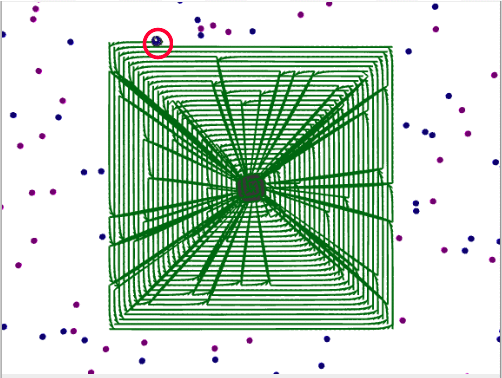
\includegraphics[scale = 0.175, width=0.4\textwidth, height =0.2\textwidth]{Figure1.png}}{\caption{\small A robot (circled red) performing the DSA. The nest is gray and path is green.}\label{DSA}}
            \vspace{-2pt}
            \ffigbox{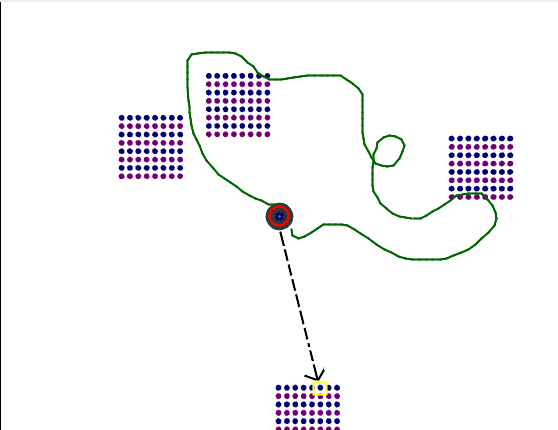
\includegraphics[scale = 0.175, width=0.4\textwidth, height=0.2\textwidth]{Figure2.png}}{\caption{\small A robot preforming the CPFA. Pheromone trail is black, next target is circled yellow, and the random walk is green.}\label{CPFA}}
          \end{floatrow}
       \end{figure}\vspace{-12pt}

%%%%%
%Body text continues
%%%%%

\vspace{10pt}
\noindent {\textbf{Methods and Results: }}We ran each algorithm 50 times for 1 hour real time trials, for multiple resource placements for each search algorithm. We observed the number of resources collected per hour in random (Fig. 1) and clustered (Fig. 2) distributions. Our results reveal that the CPFA and DSA do equally well when collecting randomly distributed resources, and that the DSA outperforms the CPFA by an average of 54\% when a single robot collects resources clustered in the large piles shown in (Fig. 2). 
\noindent This outcome aligns with our prediction that DSA will outperform the CPFA with a single robot because the advantage of being a pre-planned bounded exhaustive search that eliminates repeated steps unlike the repeated and random search from the CPFA. We expect that the CPFA will improve relative to the DSA as we increase the number of robots because communication among robots has previously been shown to improve the CPFA.  \\
\noindent {\textbf{Conclusion: }}We will illustrate the performance of the DSA and the CPFA  given different swarm sizes and resource distributions. Future work will incorporate obstacles and localization error in order to observe the effect of error on the DSA. This will test our prediction that DSA is a reliable and efficient search algorithm for foraging swarms without error, but that the CPFA is superior given large numbers of robots with localization error.

%%%%%%
%References
%%%%%%
\noindent
\vspace{-5pt}
\renewcommand\refname{} 
\vspace*{-1.5cm}
\begingroup
\bibliographystyle{plainnat} % or try abbrvnat or unsrtnat
\bibliography{example} % refers to example.bib
\endgroup


\end{document}